% crossref 
%\externaldocument{../chapter_2_methods/chapter_methods}
%\externaldocument{../chapter_3_habitats/chapter_habitats}
%\externaldocument{../chapter_4_competition/chapter_competition}


\chapter{Discussion}

The work I am presenting in this thesis was largely inspired by the natural behavior of \lepto{} we observed during a field trip to Colombia in 2016 in the context of my master thesis. Since to this time, field studies on electric fish were rare and the development of precise hypotheses was accordingly complicated, we simply recorded the electric signals of present fish continuously for a period of two weeks using a grid of 64 electrodes. Back in the lab, we developed and tested different hypotheses while analyzing the recorded data. The on-site experiments of our field trip, including recordings with simple handheld devices, i.e. transect recordings, suggested \lepto{} to coexist in high densities in the wild. Accordingly, we expected to observe a multitude of behaviors that can be associated with the social life of these fish. However, when we started to analyze the data, we were overwhelmed by the large number of recorded fish and the complexity of their behaviors. We detected up to 26 fish in about 3.5\,m$^3$, exceeding our expectations by magnitudes and significantly complicating reliable signal tracking. The applied algorithms only provided rather fragmentary EODf traces with many flawed connections and therefore required extensive manual corrections (\figref{Colombia_traces}). Nevertheless, I was able to gain preliminary insights into the fish's natural spatio-temporal and even electrocommunication behavior.

\begin{figure}[h!]
  \centerline{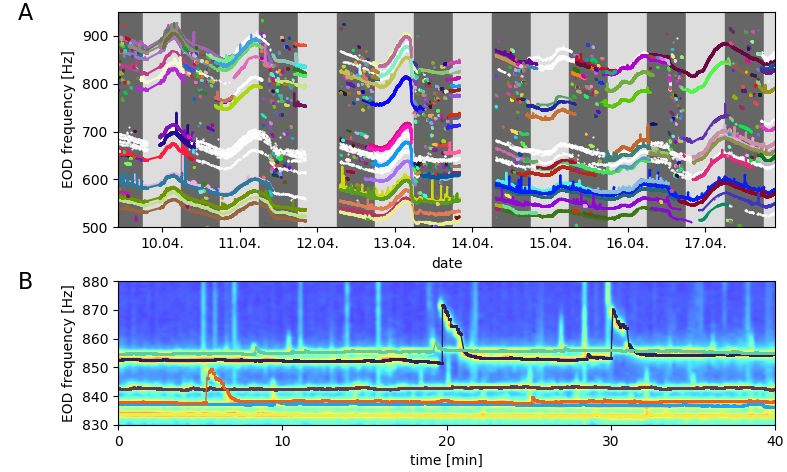
\includegraphics[width=1\textwidth]{traces}}
  \caption{\label{Colombia_traces} Long-term field recording of \macros{}, a member of the \lepto{} species group, in Colombia, 2016. EODs were recorded with a 64 channel electrode array covering $3.5 \times 3.5$\,\meter\squared. \figitem{A} Eight days of EODfs detected and tracked. Each reliably detected fish is indicated in a different color. Unreliable detections for which we need to further improve our algorithms are indicated in white. Dark gray areas indicate night time, light gray areas day time. \figitem{B} Spectrogram of a 40 minute long section of the recording from April 14$^{th}$, 2016 with tracked EODf traces. EODf traces frequently cross each other when fish emit rises as electrocommunication signals.}
\end{figure}

The tracking issues that arose from the complexity of electric recordings obtained in the wild encouraged me to improve tracking algorithms in cooperation with Noah Cohen's Lab at the Johns Hopkins University in Baltimore, USA (\chapref{Methods}). These improvements were crucial for evaluating the complex electric long-term recordings obtained in subsequent experiments (and in the wild) since they reduced the expense of extensive EODf trace post-processing. Furthermore, the behavioral complexity we observed in the wild clearly indicated the necessity for elaborate laboratory experiments to first gain understanding of the different aspects of the natural social life of \lepto{}, including the causalities of associated behaviors, before being able to make sense of the complex behavioral data contained in field recordings. 


%Furthermore, the behavioral complexity we observed in the wild clearly indicated the necessity for elaborate laboratory experiments in order to understand the different aspects of the natural social life of \lepto{}, including the causalities of associated behaviors, and then be able to make sense of the complex behavioral data contained in field recordings. 
%
%Furthermore, the behavioral complexity we observed in the wild clearly indicated the necessity for elaborate laboratory experiments. In order to make sense of the complex behavioral data contained in such recordings, we first need to gain understanding of the different aspects of the natural social life of \lepto{}, including the causalities of associated behaviors.

Consequently, my thesis pursued two main objectives: (i) The development of an algorithm capable of tracking individual EODs in various electrode array settings and (ii) the utilization of this technique in different behavioral experiments aiming to advance our knowledge about the different aspects of the social life of \lepto{} and the causalities of associated behaviors. Ultimately, these objectives aimed towards better understanding of its behaviors observed and recorded in the wild that, without knowledge gained from laboratory studies, would remain difficult to interpret.

In \chapref{Methods}, a semi-automatic system capable of tracking individual EODs based on individual-specific EOD features is presented. The algorithm combines previous approaches of tracking either the individual-specific EODf \citep{Henninger2020} or the spatial properties of an individual's electric field \citep{Madhav2018}. Furthermore, it has been inspired by the general approach of biometric systems, i.e. detecting specific manifestations of an animal's behavior or appearance (biometric entities) in order to classify them according to predefined biometric profiles, which correspond to typical manifestations of these biometrics in, for example, a certain species, individual, or behavior \citep{Gaston2004, Sherley2010,  Kuhl2013}. These advancements considerably increased tracking accuracy and reduced the effort of post-processing tracked EOD traces. Accordingly, the algorithm facilitates the evaluation of complex multi-electrode recordings, enabling large-scale studies on freely moving and interacting electric fish populations, even in high densities. 

The development of this advanced tracking algorithm was a requirement for the experiments described in \chapref{Habitats}~\&~\ref{Competitions}. Utilizing these techniques, we were able to monitor and characterize individual spatial-temporal behaviors within a group of 14 \lepto{} over 10 consecutive days (\chapref{Habitats}, \citealp{Raab2019}). In this experiment, fish have been housed in a large communal tank (2m$^3$ water capacity), stocked with several naturalistic habitats inspired by their natural environment observed in Colombia (\subfigref{eodtraces}{A, B}). The evaluated movement patterns suggest fish to mainly distribute independently from each other according to the presence of suitable shelters (\subfigsref{eodtraces}{E}, \subfref{habitatpref}{C}). Interestingly, individual diurnal activity patterns correlated with EODf. In male \lepto{}, higher EODf has previously often been associated with dominance \citep{Hagedorn1985, Dunlap2002, Triefenbach2008}. In our study, males with higher EODf showed enhanced explorative behavior during the night and increased territoriality during the day (\subfigref{transitions}{B}), which both could represent manifestations or displays of dominance. Females, on the other hand, have previously been suggested to form no dominance hierarchy at all \citep{Hagedorn1985} or only a less pronounced one, causing females with higher EODf to be more likely found inside of shelter-tubes \citep{Dunlap2002}. In our study, we found females with higher EODf to be more active during both day and night (\subfigref{transitions}{B}), suggesting EODf in females to indicate more active character traits rather than dominance. 

In a subsequent study, we evaluated behaviors and interactions of unfamiliar pairs of \lepto{} during staged competitions (\chapref{Competitions}, \citealp{Raab2021}). Fish with larger body size usually won competitions, i.e. occupied the superior shelter during the light phase at the end of the trial (\figref{bodysize}). EODf and sex played a secondary role at best (Table~\ref{glm_table}). During the dark phase of each trial, fish showed typical competition behaviors in terms of ritualized fighting supplemented by electrocommunication with rises (\figref{trial}). Rises were almost exclusively emitted by losers (\subfigref{EODfriserates}{A, B}), whereas agonistic interactions were exclusively initiated by winners. The number of rises emitted by losers and the duration of chase behaviors depended in similar ways on the contestants' physical attributes. Detailed evaluations of these correlations suggest \lepto{} to adjust their competition behavior according to mutual assessment \citep{EnquistLeimar1987} and males to presumably be more motivated to win competitions \citep{ArnottElwood2008}. Rises seemed to be costly in terms of increasing the probability to trigger winners into initiating agonistic actions and to be chased for a longer time period (\figref{event_rises}). Regardless, losers continued to emit rises even after the winner of a trial was, according to a clear difference in communication behavior, already determined (\subfigref{EODfriserates}{C, D}). Since both rise quantity and average duration of agonistic interactions increased with decreasing difference between the contestants' RHP (\subfigsref{risefactors}{C}, \subfref{agonistics}{C}), i.e. according to mutual assessment, we suggest rises to signal a loser's motivation to continue assessment, ultimately aiming to reduce relative dominance and alter the skewness in general access to resources in its favor \citep{Sapolsky2005}. Interestingly, males who lost against females seemed to be additionally motivated to continue assessment. In the respective trials, males emitted rises at high rates despite of large RHP differences to the winning females (\subfigref{risefactors}{A, C}).

Our studies demonstrate the capability of the developed algorithm to track electric signals of individual electric fish, including electrocommunication signals, even in complex long-term grid recordings (\chapref{Methods}). This technique enabled us to obtain a plethora of unadulterated behavioral data on freely moving and interacting \lepto{}. By evaluating the observed behaviors in the context of common competition and dominance theories, we have advanced our knowledge about the secretive social life of \lepto{} and set the stage for the success of future behavioral studies on the natural behavior of electric fish, including the analysis of complex recordings made in the wild. 

\section{Implications for data processing}

The technological advances of the last decades greatly increased our capabilities to study natural and undisturbed animal behaviors across various species \citep{Hughey2018, Jolles2021}. A common technique to monitor animals and their behaviors in their natural habitats is the utilization of bio-loggers, i.e. small animal mounted devices, equipped with different sensors (e.g. \citealp{Strandburg2015}). An alternative approach is to detect animals and their behaviors in external recordings, e.g. obtained with remote sensing devices like drones equipped with different sensors, or directed stationary camera-, microphone-, or electrode-setups \citep{Anderson2014, Dell2014, Hughey2018}. Each technique, however, comes with different challenges for data processing and handling. For example, external recording devices provide rather unspecific data that requires extensive processing in order to obtain reliable and exploitable behavioral data (e.g. \citealp{Kuhl2013, Dell2014}).

Likewise, our approach of recording electric signals of freely moving electric fish using arrays of recording electrodes provided rather unspecific data, too. In order to derived distinct behavioral traces for individual fish from our data, we pursued and adapted the approach of an animal biometric system \citep{Kuhl2013}. Commonly, this approach involves pattern detection and classification by means of machine-learning or deep-learning algorithms. Specific animal biometrics, i.e. manifestations of an animal's behavior or appearance, are classified by comparing them to predefined biometric profiles, i.e. typical manifestations of a respective tracking category, like species, identity, or a certain behavior \citep{Burghardt2006, Sherley2010, Ernst2011}. However, this method only provides reliable results with static biometric profiles that show little to no overlap in their definite characteristics. 

Being restricted to EOD characteristics, biometric profiles corresponding to individual electric fish are rather unspecific. Spatial electric field properties change with a fish's movement \citep{Madhav2018} and its EODf in the context of communication \citep{Zupanc2002, Triefenbach2008, Smith2013}. This variability results in potentially overlapping EOD features between individuals that consequently can lead to tracking errors. Nevertheless, each of these EOD features itself have formed the basis of one of the previous tracking approaches \citep{Madhav2018, Henninger2020}. Since both approaches track signals consecutively according to their temporal detection, their tracking accuracy further decreases for data sections where signals of single fish are temporarily not detected (e.g. detection losses caused by too large distances to recording electrodes). Both approaches achieve high tracking accuracy when evaluating low density fish populations. However, with increasing abundance and accordingly increasing overlap of individual EOD features (smaller EODf differences and similar locations of multiple fish), tracking issues accumulate and accuracy decreases respectively.

To circumvent these issues, we partly detach the tracking process from the temporal detection of signals. Instead of tracking signals in the order of their temporal detection, we identify potential signal pairs in 30\,second tracking windows and link them in a succession of decreasing signal similarity (\figref{tmp_tracking}). Consequently, we not only avoid tracking errors caused by temporal signal detection losses, but also ensure signal traces to be generated according to the highest similarity between signal pairs. Additionally, our algorithm benefits from utilizing a combined signal error comprising both EODf and spatial field property difference for tracking individual EOD traces. Rapid changes in one of these signal features, e.g. caused by rapid movements or the emission of a communication signal, can be compensated by the respective other signal feature, whereby tracking errors can be avoided.

Despite our advancements in tracking accuracy, sporadic manual corrections of flawed EODf traces remain necessary. In its current state, the presented algorithm establishes new signal pair connections solely based on their similarities. Indeed, even better tracking results could be achieved by implementing signal trace predictions that dynamically adapt to already established connections within a current tracking segment. Corresponding implementations, however, would require an even more dynamic tracking algorithm and multiply the required computational power and time beyond efficient scientific feasibility. In future studies, a neural network could be trained on tracking individual EODf traces, similar to existing pose detection algorithms (e.g. \citealp{Mathis2018}). Such approaches, however,  require extensive training data-sets in order to perform with reliable accuracy. Accordingly, our algorithms and evaluated data-sets might represent the basis for the development of such an even more advanced tracking system in the future.

In conclusion, our developed algorithm not only improves tracking accuracy of wave-type electric fish compared to previous approaches \citep{Madhav2018, Henninger2020}, but also advances the general approach of biometric systems \citep{Kuhl2013}. By refraining from static biometric profiles and rigid classifications in favor of probabilistic time-variant classifications, we enhanced the general applicability of this method. Our method relies only on the extraction of specific features suitable for describing a tracking category in external recordings. In our case, this corresponds to EOD features extracted from electrode grid recordings and used for tracking electric signals of individual fish. However, since these tracking features can be anything detectable in external recordings of any modality, our method is not limited to tracking electric fish alone, but can also be adapted to tracking tasks across various animal species, or even beyond behavioral studies or science in general. 

A major benefit of machine-aided analysis is its capability to process enormous amounts of data (mainly automatically). This is not only useful to solidify specific scientific statements \citep{Gomez2014, Dell2014}, but also enables important explorative studies. In our case, machine-aided analysis was crucial to enable our explorative recordings of populations of \lepto{} in their natural habitats in Colombia. Even though at the time, we were unable to understand the specific significance and causalities of observed behaviors, these field trips led to specific hypotheses and the development of the laboratory experiments described in \chapref{Habitats} and \ref{Competitions} and further discussed below. 

\section{Implications for the social life of \lepto{}}

Behavior does not occur in a contextual vacuum \citep{Rendall1999, Seyfarth2017, Henninger2018}. Accordingly, in order to understand the meaning and causalities of specific behavioral events, a detailed understanding of the framework in which behaviors occur is vital (e.g. \citealp{Rendall1999, Henninger2018}). A crucial aspect shaping the scope of possible interpretations of social behaviors is the structure and organization of an animal's social environment. For example, specific communication signals in group living species can frequently be associated with behavioral coordination or cooperation (e.g. group cohesion, \citealp{Demartsev2018}, collective anti-predator defense \citealp{Schibler2007}; reconciliation, \citealp{Cheney1995}, etc.). However, for solitary species, a coherence between communication and mate attraction or agonistic actions is way more likely, simply because of their respective way of life \citep{Cornhill2020}. 

The social organization of \lepto{} has rarely been addressed in previous studies. For other electric fish species, primarily those belonging to the family of African \textit{Mormyrides}, different behavioral patterns have been identified suggesting them to be live in social groups. Some electric fish species form shoals (e.g. \textit{Mormyrus rume proboscirostris}, \citealp{Worm2021}, \textit{Mormyrops anguilloides}, \citealp{Arnegard2005}, or \Eigenmannia, \citealp{Oestreich2005}), emit communication signals that can be associated with group cohesion \citep{Arnegard2005, Worm2021}, and even forage or hunt collectively in a group \citep{Arnegard2005, Bastos2021}. 

For \lepto{}, corresponding observations are sparse. In the laboratory, \lepto{} distribute independent from each other according to the availability of suitable shelters (\subfigref{eodtraces}{E}, \subfref{habitatpref}{C}). Similar observations have also been made in the field (own observations in Colombia, 2016, 2019, \citealp{Stamper2010}). On the other hand, in a forced choice experiment \citet{Stamper2010} observed \lepto{} to reliably approach tubes with EOD mimics of con-specifics instead of non-stimuli tubes. However, considering that \lepto{} shows increased aggression towards con-specifics compared to other electric fish species (e.g. \citealp{Triefenbach2008}), this approaching behavior is presumably rather associated with initial assessment and competition than with the intention of shoaling. 

Nevertheless, Gymnotiform fishes, including \lepto{}, make up to 70\,\% of the biomass of large rivers in South America \citep{Marrero1991, Cox2004, Crampton2011}. Therefore, frequent interactions with con-specifics are inevitable. We ourselves observed high densities of \lepto{} in a small river in Colombia (up to 26 individuals in about 15\,m$^2$, \subfigref{Colombia_traces}{A}). However, neither ourselves nor other studies observed or reported individual behaviors as evidence for \lepto{} to be a group living species, e.g. collective movement or cooperation. Therefore, we suggest \lepto{} to actually be a rather solitary living species that is forced to share its habitat with con-specifics because of their high abundance. Yet individual fish could benefit passively from the presence of con-specifics, e.g. by means of an overall reduced individual predation risk or increased reproductive success \citep{Cote1995, Clutton-Brock1999, Sword2005, Bilde2007}. On the other hand, fish also have to face the challenges arising from increased intra-specific rivalry for limited resources (e.g. \citealp{Janson1985, Chapman1995, Markham2017}). The diversity of social interactions in \lepto{} we observed and evaluated in the process of this thesis could have been developed in order to facilitate the frequent social encounters and interactions that inevitably result from their high abundance in natural habitats.

%\subsubsection{Behavioral interactions in \lepto{}}
\subsection{Assessment during competitions in \lepto{}}

\begin{figure}[h!]
  \centerline{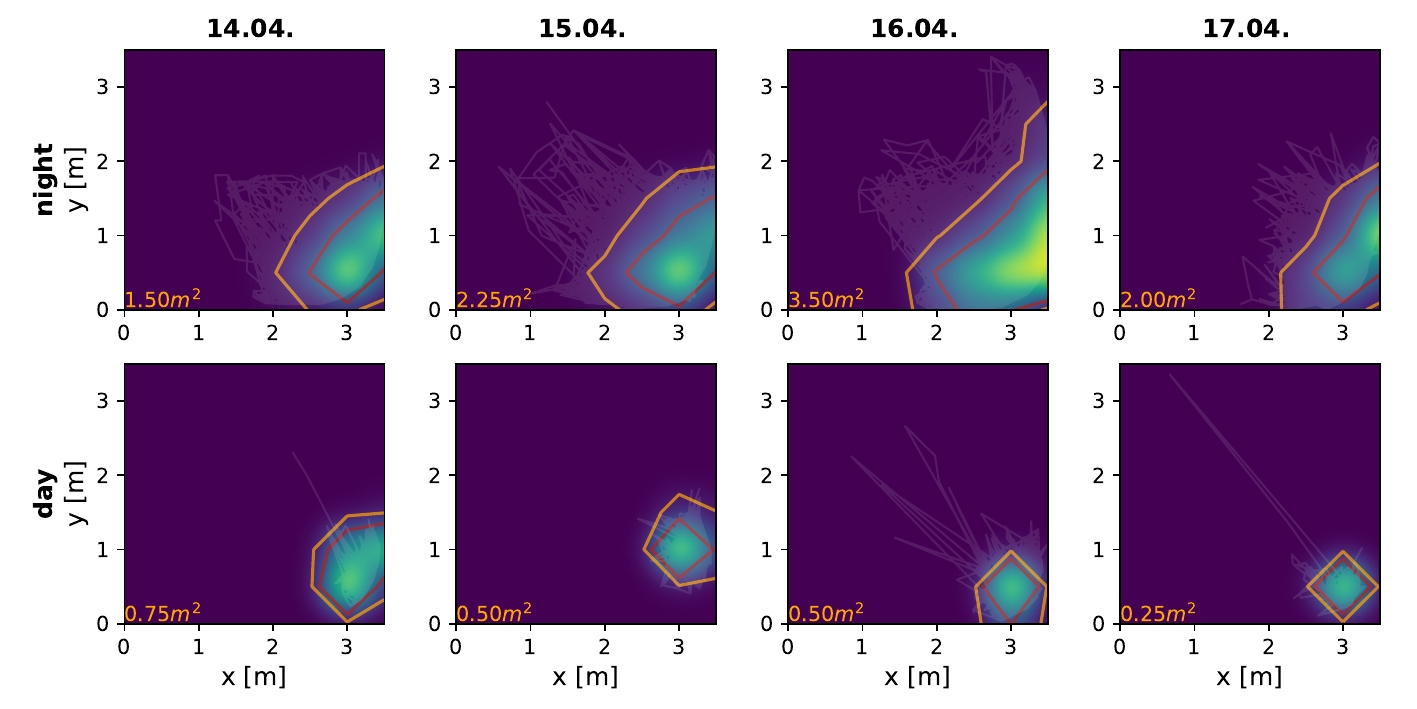
\includegraphics[width=1\textwidth]{stationary_jpg}}
  \caption{\label{Colombia_stationarity} Spatial behavior of a single \macros{} detected and tracked consecutively for four days. Heat-maps and contour lines show the fish's probability of presence across the monitored 3.5$\times$3.5\,m$^2$ area of the river during the night (top panels) and day (bottom panels). Orange contour lines include the area in which the fish spends more than 50\,\% of the time, the red lines more than 75\,\% of the time respectively. Even though the fish certainly shows movement behaviors, especially during the night, it remains remarkably stationary in the bottom-right corner of the observation area for four consecutive days.}
\end{figure}

In the presence of con-specifics, animals frequently rival for limited resources and fighting is usually a key behavior to secure access \citep{Cluttonbrock1979, Chapman1995, Markham2015}. However, competition is costly in terms of time and energy allocated to it and an increased risk of injury or death (e.g. \citealp{Briffa2004}). In order for competitions to be evolutionary stable, potential benefits always need to outweigh the associated costs \citep{ArnottElwood2009}. Accordingly, different species developed various mechanisms to economize competitions, e.g. specific assessment strategies \citep{EnquistLeimar1987, Payne1998, Taylor2003} or a dominance hierarchy to regulate access to resources (e.g. \citealp{Janson1985, Sapolsky2005}). Which mechanism eventually manifests in a given species, depends on its social organization and given environmental situations. The development of a complex dominance hierarchy is most beneficial if repetitive rivalry with the same individuals is likely. Developing elaborated assessment strategies can be useful when animals frequently compete with the same as well as different individuals. When competitions are rather scarce or resources are abundant, presumably neither of these mechanisms will develop because the costs of developing associated behaviors are not covered by the resulting benefits.

In order to understand how \lepto{} resolves conflicts, we evaluated their competition behavior during staged competitions (\chapref{Competitions}, \citealp{Raab2021}). Competitions were usually won by the larger individual, suggesting resource holding potential (RHP, \citealp{Parker1974}) in \lepto{}, i.e. an individual's potential to inflict and endure damage \citep{Archer1988}, to be primarily based on body size. In our experiments, additional factors influencing the outcome of competitions, like positional advantages, were intentionally eliminated by the experimental design. However, in the fish's natural habitats, where we observed highly stationary fish (Colombia, 2016, \figref{Colombia_stationarity}), positional advantages of a resident could still bias competitions to be rather won by residents than intruders, as observed in other species (e.g. \citealp{Alcock1997}). 

In some species, animals actively assess their individual chances of winning competitions by interpreting passive cues and active signals which indicate their opponent's fighting motivation and capability \citep{Cluttonbrock1979, EnquistLeimar1987}. This information exchange can often already be sufficient to resolve conflicts without the necessity of costly escalating physical fighting \citep{Parker1974, Cluttonbrock1979, Jason1990}. In \lepto{}, observed competitions comprised ritualized fighting \citep{Triefenbach2008} accompanied by rises as electrocommunication signals \citep{Smith2013}. Agonistic events were initiated by the winners of trials whereas rises were primarily emitted by the respective losers. Both behaviors occurred with unvarying frequency within trials, and their extent similarly increased with decreasing size difference between competitors. This suggests (i) behavioral decision making in competitions between pairs of \lepto{} to be based on mutual assessment and (ii) both ritualized fighting events and rises to be important in terms of information gathering during this process. These conclusions, again, match with our observations made in the fish's natural habitats. As aforementioned, \lepto{} can be found in high densities in the wild. However, at the same time we only found little food items in the corresponding clear streams. With many fish to compete over sparse high value resources, the development of behaviors associated with mutual assessment is reasonable and the most economic approach to resolve the corresponding conflicts \citep{ArnottElwood2009}.

\subsubsection{Electrocommunication with rises}

Our competition experiment suggests rises to be emitted by losers in order to signal their motivation to continue assessment. Thus, during competitions, rises can be assumed to be an important signal to gain valid information about a con-specific in the process of mutual assessment. Accordingly, their emission should be net beneficial and evolutionary stable, even though they are costly in terms of increasing chances of being attacked or chased for a longer time period (\figref{event_rises}). However, rises are rather generic signals. They show huge variations in terms of duration (lasting from seconds up to many minutes) and EODf increase (up to 68\,Hz). In some configurations, rises can potentially even be confused with other active EODf modulations observed in \lepto{}, e.g. a short jamming-avoidance response \citep{Tallarovic2005}. The structural variability of rises indicates that they are rather unspecific signals with little informative value \citep{Seyfarth2003}. We suggest the specific meaning of rises to arise from the behavioral context they are emitted in \citep{Seyfarth2003}. During competitions, rises seem to signal motivation \citep{Raab2021}. Further applications of rises in various behavioral contexts could potentially be revealed in detailed observations of whole populations of \lepto{} under more naturalistic conditions.

\subsection{Implications on the social hierarchy in \lepto{}}

Even though elaborate assessment strategies can economize competitions \citep{ArnottElwood2009}, costs still accumulate when animals rival with the same individuals over and over again. To further economize these rivalries, some species fight in order to establish dominance hierarchies, where an animal's access to resources is determined by its social status (e.g. \citealp{Wauters1992, Sapolsky2005, Taves2009}) and mutual knowledge about hierarchical ranks prevents repetitive fights among familiar individuals \citep{Cluttonbrock1979, Fernald2014, Cornhill2020}.

Dominance hierarchies have also been suggested for various electric fish species \citep{Westby1970, Fugere2011, Silva2012}, including \lepto{} \citep{Hagedorn1985, Dunlap2002, Stamper2010, Henninger2018}. Previous studies suggest that male but not female \lepto{} form a dominance hierarchy \citep{Hagedorn1985, Dunlap2002}. More dominant males have been reported to occupy higher quality shelters, preferably alone \citep{Dunlap2002}, and to show increased participation in reproduction \citep{Hagedorn1985, Henninger2018}. Females, on the other hand, have been suggested to either form no dominance hierarchy at all \citep{Hagedorn1985}, or only a distinct one, whereby less dominant females are more likely to be found outside of shelter tubes \citep{Dunlap2002}. 

As discussed above, we suggest \lepto{} to actually prefer remaining solitary over living in groups, even though they are forced to share their natural habitats with con-specifics because of their high abundance. Dominance in \lepto{} can therefore be assumed to be rather resource based, as in other solitary species (e.g. \citealp{Cigliano1993}), instead of coming along with complex social structures and group behaviors, like, for example, the development of a leader-follower dynamic \citep{Strandburg2018}. Accordingly, determining whether the social life of \lepto{} is shaped by a social hierarchy or repetitive competitions over resources is complicated in experiments with short observation times, but can potentially be answered by interpreting individual behaviors in long-term observations. 

As aforementioned, we found \lepto{} in abundance in the wild where individuals frequently remained rather stationary over several days (\figsref{Colombia_traces},\fref{Colombia_stationarity}). Accordingly, frequent interactions and rivalry with the same individuals are inevitable and the development of a dominance hierarchy would be the most efficient way to distribute resources and reduce the necessity of repetitive costly fights \citep{Sapolsky2005}. Further support for the social life of \lepto{} being shaped by a dominance hierarchy instead of fighting in repetitive competitions arises from their observed communication behavior. Rises have only occasionally been observed in the wild and their quantity seemed to decrease throughout the two weeks of our first laboratory experiment (\subfigref{eodtraces}{C}). Since we could further show that rises are reliably emitted in the context of competition between pairs of \lepto{} \citep{Raab2021}, this suggests competitions to be rather sparse in the wild and to decrease over time in artificially compound populations. Consequently, rises and competitions can be assumed to be mainly used to establish dominance during initial encounters, which then regulates access to resources and prevents the high costs of repetitive fighting.

\subsubsection{Skewness of the social hierarchy in \lepto{}}

In our competition experiments, dominance is attained through agonistic interactions and resources are claimed entirely by dominants. At first glance, this suggests a despotic dominance hierarchy for \lepto{} \citep{Kappeler2008}. On the other hand, these agonistic interactions resemble non-escalating ritualized fights \citep{Triefenbach2008} which are often used to intimidate con-specifics and obtain or maintain dominance in rather egalitarian hierarchies across species \citep{Sapolsky2005}. Furthermore, we did not observe active displacement from micro-habitats in our first group experiment, indicating fish to tolerate the presence of con-specifics and, consequently, to share available resources. We suggest our contradictory observation of fish monopolizing resources in our competition experiments to result from the very limited resources in this experiment that could hardly be shared anyway. Further support for more egalitarian dominance hierarchies in \lepto{} comes from their observed communication behavior during staged competitions. Losers continued to emit rises at a constant rate and thereby stimulated agonistic attacks, even though the outcome of competitions was presumably already set and mutually recognized within the initial phase of interactions. However, continued mutual assessment could be used to adjust relative dominance between competitors and thereby the skewness in access to resources, which can be assumed to be obsolete in despotic hierarchies. Finally, our hypothesis of a rather egalitarian hierarchy in \lepto{} is further supported by the preliminary observation of multiple males participating in reproduction in the wild \citep{Henninger2018}. 

\subsubsection{EODf as signal of dominance}

In order for dominance hierarchies to economically resolve conflicts between con-specifics, individuals need to be able to assess each other's social status. Accordingly, different species developed specific signals conveying corresponding information \citep{Cluttonbrock1979, Fernald2014, Cornhill2020}. When fish are not in each other's direct proximity, \lepto{} can exclusively exchange information with con-specifics using their EODs \citep{Knudsen1975, Henninger2018, Henninger2020, Benda2020}. Therefore, these electric signals would be most suitable to signal dominance in \lepto{}. Indeed, some studies found dominance to correlate with EODf in males, and to some extend also in females \citep{Hagedorn1985, Dunlap2002, Triefenbach2008}. Furthermore, in males EODf has sometimes been found to correlate with body size \citep{Dunlap2002, Triefenbach2008}. 

In our competition experiments we did not find a correlation between body size and EODf in either sex. Nevertheless, the accuracy of our generalized linear model predicting winners of competitions increased slightly when including EODf as an additional parameter besides body size (\figref{glm}). Furthermore, we clearly found EODf dependent spatio-temporal movement traits for both sexes in our first laboratory experiment, which, at least for males, can also be associated with dominance or corresponding displays (\subfigref{transitions}{B, D}). Both our own observations as well as the inconsistency across studies in finding a link between EODf and body size or dominance suggest EODf to be, at best, an unreliable predictor for dominance. Nevertheless, as aforementioned, the EODs of electric fish are the only source of information that can be accessed by con-specifics from afar. Accordingly, EODf could be used as an initial rough estimate of a potential opponent's body size, RHP, or dominance. 

As discussed above, we suggest rather egalitarian dominance hierarchies for populations of \lepto{}. In this kind of social organization, the evolutionary pressure to compete with con-specifics can be expected to be reduced in comparison to despotic hierarchies. Accordingly, validating the rough dominance estimate obtained from a potential competitor's EODf by approaching them and risking physical competition could be too costly to outweigh the potential benefits. \lepto{} could therefore rely on EODf as a signal of dominance when the availability of resources is generally sufficient and fish mainly perceive each other electrically, e.g. in our first open space laboratory experiment or in the wild.

\section{Sexually dimorphic behavioral traits}

In our experiments, we repeatedly found sexually dimorphic behavioral traits. For males, we could identify distinct movement behaviors that can be associated with dominance or interpreted as corresponding displays, i.e. territoriality at shelters during the day and increased exploration behavior during the night (\subfigref{transitions}{B, D}). Furthermore, the correlation between larger body size and winning staged competitions was stronger in males compared to females (\subfigref{bodysize}{B--E}) and males emitted an especially high number of rises when losing against larger females (\subfigref{risefactors}{A, C}). Together with previous observations of males showing increased territoriality \citep{Dunlap2002} and increased overall aggression towards con-specifics compared to females, this suggests a generally boosted motivation in males to win competitions and gain or maintain dominance. These motivational differences could explain the observed behavioral divergences between males and females \citep{ArnottElwood2008}.

% boosted motivation in males
In our experiment, we could not clearly determine the cause for the suggested motivational differences between the sexes and the resulting sexually dimorphic behavioral traits. However, since access to different limited resources, e.g. food, shelter, etc. is usually  determined by an animal's social status \citep{Janson1985, Blumstein2001, Charpentier2005, Dunham2008}, we suggest a sexually dimorphic valuation of these resources to be a possible cause for the respectively observed behavioral differences in \lepto{}. 

Although \lepto{} is sexually quite monomorphic, which suggests requirements for food or shelter and their valuation to be rather similar for both sexes, a possible divergence could arise from \lepto{} mating behavior. During the mating season, males are known to compete for females, which after an extensive mating ritual spawn a single egg in a location save from external threats such as strong currents or predators. Under the assumption that females assess the quality of a male by assessing the suitability of its shelter for reproduction, shelters could be some kind of secondary sexual characteristic of males and therefore increase their motivation to compete for them. Nevertheless, it should be noted that in \rostratus, a close relative of \lepto{}, preliminary observations suggest males to visit females in the context of mating, rather than \textit{vice versa}, which contradicts our hypothesis.  


% dominance in females 

\subsection{Females in the dominance hierarchy of \lepto{}}

As discussed above, the observed behavioral traits of females in our experiments suggest them to be less eager to prevail in social contexts. Contrary to males, we did not find movement behaviors that can be associated with dominance or corresponding displays and body size was less predictive for winning competitions. These observations are consistent with previous studies suggesting females to be overall less aggressive and more tolerant towards the presence of con-specifics compared to males (e.g. \citealp{Dunlap2002}). Accordingly, the only competition trial in which we observed both contestants sharing the superior shelter in the end was won by a female (the other contestant was male; loser identified by rise quantity). Altogether, the more peaceful and passive behavioral characteristics suggested for females could, indeed, be associated with them not forming a dominance hierarchy as suggested in previous studies \citep{Hagedorn1985, Dunlap2002}. 

On the other hand, fish of both sexes showed similar (even though not identical) competition behaviors during our staged competitions. Another possible yet still rather hypothetical and uninvestigated explanation could be that females are evolutionary less reliant on dominance and associated benefits. The rather egalitarian dominance hierarchy previously suggested for \lepto{} in this thesis, could generally provide sufficient resources for females and limit their active participation in dominance fights to occasions where resources are scarce, e.g. in our competition experiments.

\section{Open ends and perspectives}

In the presented thesis, I demonstrate how extensive behavioral observations in an animal's natural environment can lead to specific scientific questions and the development of elaborate techniques and complex laboratory experiments in order to answer them. In our case, we developed tools, techniques, and laboratory experiments to advance our knowledge about the behavioral adaptations in \lepto{} which enable them to successfully inhabit their natural habitats in high densities.

% competition
Our results suggest \lepto{} to economize the frequent conflicts inevitably resulting from their high abundance in the wild through mutual assessment. By means of ritualized fighting and information exchange via electrocommunication, contestants gather information about each other's resource holding potential and adapt their behavior according to the disparity. In this process, rises seem to be important signals to coordinate competitions. With their emission, subordinates seem to signal their motivation to continue assessment by stimulating ritualized fighting. In order to further increase our knowledge about the different social aspects of competitions in \lepto{}, we plan to adjust the experimental design of future competition experiments to enable the additional detection and evaluation of chirps. In previous studies, these communication signals have already been associated with agonistic interactions and could therefore reveal further details of the fish's competition behavior when included in our analysis. 

% social organization in \lepto{} - how to verify it ?
The evaluation of individual behavioral traits and social interactions of \lepto{} in the context of this thesis provides a strong basis for developing hypotheses regarding the overall social structure in populations of \lepto{}. Together with our observations from the field, the conclusions of our laboratory experiments indicate \lepto{} to (i) develop dominance hierarchies, where (ii) an individual's access to resources is proportional to its social status, and (iii) males are more motivated than females to gain dominance and associated benefits.

Even though all of our conclusions derive from elaborate and detailed behavioral observations, some assume still unverified causalities and therefore require further scientific validation. Accordingly, future experiments should increase in complexity and gradually approximate natural conditions in order to create experimental setups where these questions can potentially be answered. For example, detailed observation of competitions and associated behaviors in small groups of \lepto{} competing over divisible and measurable resources (e.g. distributed small food items or shelters of varying quality as in \citealp{Dunlap2002}) could help to clarify the skewness in access to resources across the dominance hierarchy in populations of \lepto{}. Furthermore, such elaborate experiments could potentially lead to the discovery of still unrevealed behavioral traits and causalities that only emerge and are observable in more complex social and environmental settings. The ultimate prove for our hypotheses could be obtained by inducing breeding conditions and evaluating individual reproductive success throughout a group of \lepto{}. However, since breeding conditions induce complex changes in an animal's behavior, corresponding experiments should be conducted only after the evaluation of individual behaviors and interactions within smaller groups in complex environments (as suggested above) have been exploited. Breeding experiments could, furthermore, reveal interesting behavioral changes that complement our understanding about the social life of \lepto{}. For example, females could become more active and motivated to win competitions because their valuation of food might increase due to increased energy demand and their valuation of shelters might increase since they correspond to save spawning sites.

% How to get back to the field ? 
As repetitively mentioned throughout this thesis, our work was inspired by the complexity of electric recordings obtained from the fish's natural habitats. With the behavioral observations of our laboratory experiments, we already developed a strong basis for identifying specific behaviors solely based on characteristic electric signal changes and associated spatio-temporal behaviors. For example, we showed that rises frequently trigger agonistic interactions that come along with high velocity movement behaviors. Both electric and spatio-temporal manifestations of behaviors can also be extracted from grid recordings of electric fish in the wild. Accordingly, further laboratory experiments could provide the basis to develop an electro-spatio-temporal ethogram of \lepto{}. Such an ethogram could then be utilized to detect specific behaviors and interactions in the wild and validate their significance and causalities in the environments these behaviors have originally evolved to.  

%\bibliographystyle{jneurosci}
%\bibliography{../journalsabbrv,../references}